\section{Limity równoległych zapytań dla zbioru FWB\_100K}

\begin{figure}[!hb]
	\centering 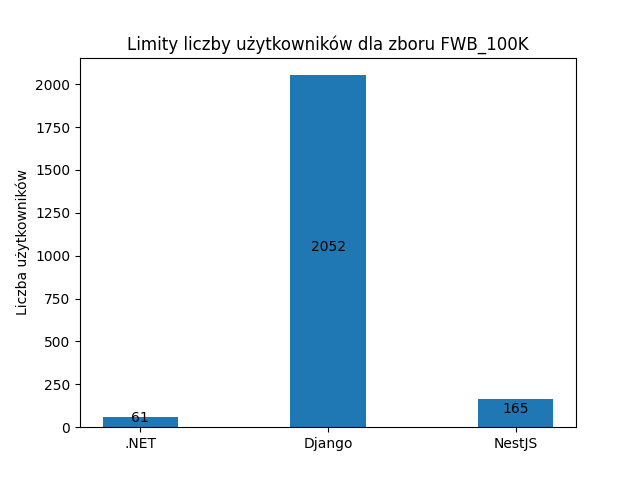
\includegraphics[width=1\linewidth]{rysunki/Limity_liczby_uzytkownikow_dla_zboru_FWB_100K.png}
	\caption{Limit liczby użytkowników przy zwracaniu zbioru FWB\_100K}
	\label{rys:limit_vus_fwb_100K}
\end{figure}

Wyniki badania limitów zostały zaprezentowane na rysunku \ref{rys:limit_vus_fwb_100K}.

Widoczna jest zmiana zależności wyników pomiędzy frameworkami.
Największą liczbę użytkowników, na poziomie 2 tysięcy, uzyskał Django.
12-krotnie mniejszą liczbę użytkowników obsłużył NestJS.
.NET obsłużył 2 krotnie mniejszą liczbę użytkowników niż NestJS.